% draft 3rd-year diploma thesis, by Nick Manini, 2019/01/03
\documentclass[a4paper,12pt]{article}
\usepackage[english]{babel} % or other languages, e.g:
%\usepackage[italian]{babel} % needs debian package texlive-lang-italian
%\usepackage[latin1]{inputenc} % to use keyboard accented characters
\usepackage[a-1b]{pdfx} % to generate valid PDFA
                 % see https://www.mathstat.dal.ca/~selinger/pdfa/ for details
\usepackage{hyperref}
\usepackage{graphicx}
\usepackage{amsmath}
\usepackage{amssymb}
\usepackage{breakurl}
\usepackage{newtxtext}
\usepackage{physics}
\usepackage[varvw]{newtxmath}
\usepackage[width=0.8\textwidth]{caption}

% page size tuning:
\setlength{\oddsidemargin}{8mm}   % Distance from the left edge -1 inch
\setlength{\textwidth}{145mm}     % Horizontal width of the standard text
\setlength{\topmargin}{2mm}       % Distance from top to PAGE'S HEAD -1 inch
\setlength{\textheight}{225mm}    % Vertical length of the page body
\setlength{\headheight}{0mm}      % Height of a box containing the head
\setlength{\parskip}{0.5mm}       % Extra vertical space before a paragraph
\setlength{\parindent}{9mm}       % Indentation at paragraph beginning
\linespread{1.12}                 % Line-to-line spacing
\renewcommand{\floatpagefraction}{.93} % for text coexisting with figs and tabs
\renewcommand{\textfraction}{0.02}% more or less equiv. to the above

\begin{document}

\title{{\bf \huge
    Simulated run in the rain }}
\author{Cristian Angelo Crespi}
\date{Farawember 33, 2399} % the exact date of graduation, when available

\makeatletter
\let\mytitle\@title
\let\myauthor\@author
\makeatother

\author{\myauthor \\
  Dipartimento di Fisica, Universit\`a degli Studi di Milano,\\
  Via Celoria 16, 20133 Milano, Italia
}

{ % heading page  -  frontespizio

  \thispagestyle{empty}

  \centerline{
    \includegraphics[width=120mm,angle=0,clip=]{UniversitasMediolanensis.pdf}
  }

  \begin{center}
    {\Large Facolt\`a di Scienze e Tecnologie\\
      \vskip 2mm Laurea Triennale in Fisica }
  \end{center}


  \vskip 15mm
  \begin{center}
    \mytitle
%    \huge \textbf{Titolazzo della tesi, if seems long\\go to newline}
  \end{center}

  {\large
    \vskip20mm Relatore:  Prof. Nicola Manini
  }

  \vskip2cm
  \hskip9cm
  \parbox[t]{7cm}
         {\large 
           \myauthor\\
           Matricola n$^\circ$ $964503$\\
           A.A. $2023$/$2024$\\
           \vskip 0.5mm Codice PACS: 92.60.jf
         }

}


\clearpage
\thispagestyle{empty} \qquad

\maketitle \thispagestyle{empty}
\setcounter{page}{1}

%---------------------------------------------------------
\begin{abstract}
The optimal velocity of running in the rain has long been discussed in the physics and mathematics community, although in practice the human body has always been represented as a simple shape such as a parallelepiped or a cylinder. In this work we use numerical simulations to find results for more complex and dynamical shapes that can represent the human body with an accuracy never reached before in this field.
\vskip0.75cm
\hskip5cm
\parbox[t]{7cm}
{
Advisor: {\it Prof. Nicola Manini}
}
\end{abstract}
%--------------------------------------------------------

\clearpage
\tableofcontents

\clearpage

%----------------------------------------------------------------------------
\section{Introduction}
%----------------------------------------------------------------------------
The question of weather it is better to run or walk in the rain is as old as time, and has proven to be a recurring topic in the mathematics and physics community in the last 50 years. Despite the quantity of articles on the topic and the large time span in which they have been produced there have been precious little improvements upon the results first found by Schwartz and Deakin \cite{Deakin} back in 1973. In that article a parallelepiped with sides parallel to the axes is used to approximate a human body running on a straight path in the presence of rain and wind, leading the following results: in the presence of a tailwind an ideal speed can exist, and it is then equal to the component of the rain velocity along the direction of the path; without a tailwind it is always better to run faster, although with diminishing returns. Since then a variety of simple geometric shapes have been considered: spheres \cite{Hailman}\cite{Bocci}, cylinders \cite{Bocci}, paraboloids \cite{Hailman}, plane surfaces \cite{Bocci} and parallelepipeds\footnote{We refer to orthogonal parallelepipeds simply as  parallelepipeds as done in previous works on the topic.} with generic orientations \cite{Bocci}. What we can see is that the shape considered can change the results considerably: in the presence of a strong enough tailwind a finite ideal speed always exists, but its value depends on the shape considered, and for some shapes an ideal speed can exist even without wind or in the presence of headwind. Because of these discordant results the need for a better approximation of the human body becomes apparent, and the only reason this hasn't been done yet is the difficulty of deriving analytical results for complex shapes, which can be circumvented by a numerical approach. A numerical approach to the problem has been already tried \cite{Kroetz}, but it too only modeled the human body as a parallelepiped, and was more focused on comparing modeling rain as raindrops placed in a cubic lattice as opposed to the more realistic case in which the raindrops are generated at random positions; as expected, the results to not differ in the two cases considered. 

In this work we consider a model of the body composed by multiple basic three-dimensional geometric shapes that move relative to each other, to which we will from now on refer to as body parts. We used  spheres, parallelepipeds and capsules\footnote{A capsule, also called a spherocylinder sometimes, is a basic three-dimensional shape consisting in a cylinder with hemispherical ends.} to model the single body parts. In particular capsules had never been studied before in this context so an analytical solution was found. 



\newpage
\section{The model}\label{model:sec}

We consider the case of a person running along a path under rain and wind. What we want to find is the ideal speed in which to move to catch the least rain possible. We shall assume the following:
\begin{enumerate}
    \item The ground is horizontal. \label{h1}
    \item the path is rectilinear. \label{h2}
    \item The raindrops all have the same size and are densely and uniformly distributed in space. \label{h3}
    \item The wind velocity is constant and the raindrops have reached terminal velocity in the wind.  \label{h4}
    \item The wind adds a horizontal component to the velocity of the rain. \label{h5}
    \item The motion of the body is composed by a translation with constant speed along the path plus a  periodic relative motion that is generally unique to each body part but shares the same period $T$. \label{h6}
    \item The velocity of the body parts due to their periodic motion is negligible compared to the velocity of the rain.  \label{h7}
    \item The path is long enough that periods of the periodic motions of the body parts are small compared to the time $t_f$ taken to traverse the path ($T << t_f$).  \label{h8}
\end{enumerate}
In all the frames of reference we will take into consideration the $x$ axis will be along the path of the body and the $z$ axis will be the vertical axis. According to assumptions \ref{h1}, \ref{h2} and \ref{h6} the body is moving with a velocity $\mathbf{v}_b = v_b\hat{\mathbf{e}}_x$, while the rain has a velocity $\mathbf{v}_r$. The $z$ component of $\mathbf{v}_r$ has to be negative because of assumption \ref{h5}, and we will refer to its absolute value as the falling velocity $v_{fall}$. We will refer to the value of the $y$ component of $\mathbf{v}_r$ as the "crosswind" $v_{cross}$. We will refer to the value of the $x$ component of $\mathbf{v}_r$ as the "tailwind" $v_{tail}$ if it is positive and to its absolute value as the "headwind" $v_{head}$ if it is negative. We will call $d$ the total length of the path to travel.

The wetness $W$ of the traveler, measured as the total volume of water that has hit them at the end of their walk, is equal to the number of raindrops hit times the volume of each drop. Thanks to our assumption \ref{h3} we can safely define an adimensional "rain density" $\rho_{rain} = N_{drop} V_{drop}/V $, where $N_{drop}$ is the number of raindrops contained in a certain volume $V$ and $V_{drop}$ is the volume of a single drop. In short $\rho_{rain}$ is the ratio between the amount of rain contained in a volume and that same volume. Let's consider the frame of reference in which the raindrops are still. In this frame the velocity of the body is $\mathbf{v}_{rel} = \mathbf{v}_r - \mathbf{v}_b$. The raindrops hit are those inside of the volume of space that our body passes through, which we will call $V_b$. We can then use the following relation to find the wetness: $W = \rho_{rain}\, V_b$. Since $\rho_{rain}$ is constant in our walk under the rain no matter the speed of the traveler our problem reduces to finding and minimizing $V_b$. As found in \cite{Hailman} for a body whose only movement is a rigid translation $V_b$ can be found with the following formula:
%
\begin{equation}\label{EqVbRig}
V_b(\mathbf{v}_{rel}) = S_b(\mathbf{v}_{rel})\  \frac{\norm{\mathbf{v}_{rel}}}{v_b} \ d
\end{equation} 
%
$S_b(\mathbf{v}_{rel})$ is the area of the projection of the body on a plane perpendicular to $\mathbf{v}_{rel}$. The only non-trivial part of the problem is then finding out the dependence of $S_b$ on $\mathbf{v}_{rel}$.
\begin{figure} 
\centerline{
\includegraphics[width=1\textwidth,angle=0,clip=]{ProjVol.png}
}
\caption{\label{Vb:fig}
Example with a sphere as the body. Its orthogonal projection on the plane perpendicular to $\mathbf{v}_{rel}$ is a disk  with area $S_b$ and $V_b$ is the volume of the resulting cylinder. Original image from \cite{Hailman}.
}
\end{figure}

We now generalize these findings for a dynamical body. Since the velocity of the body parts is small compared to the velocity of the rain \ref{h7} we can approximate the relative velocity of the body parts with the relative velocity of the whole body $\mathbf{v}_{rel}$. This way we can write the area of the projection of the whole body as depending only on the relative velocity of the whole body and of the time:  $\Tilde{S_b}(\mathbf{v}_{rel} , t)$. We can then generalize Eq. \ref{EqVbRig} by considering that $d/v_b = t_f$ and substituting $S_b(\mathbf{v}_{rel}) \, t_f$ with an integral of $\tilde{S_b}(\mathbf{v}_{rel}, t)$ over $[0, t_f]$:
%
\begin{equation}\label{EqVbDin}
V_b = \norm{\mathbf{v}_{rel}}\, \int_{0}^{t_f} dt \, \tilde{S_b}(\mathbf{v}_{rel}, t)
\end{equation} 
%
Furthermore since the time spent traversing the path is long compared to the period of the function \ref{EqVbRig} we can approximate $\Tilde{S_b}(\mathbf{v}_{rel} , t)$ with its temporal average of over the period $T$. For a dynamic body we consider then:
%
\begin{equation}\label{EqSbDin}
S_b(\mathbf{v}_{rel}) = \frac{1}{T} \int_{0}^{T} dt\, \Tilde{S_b}(\mathbf{v}_{rel} , t)
\end{equation} 
%
By using our newfound $S_b$ we can use formula \ref{EqVbDin} for dynamical bodies too, although of course this approximation holds only if assumptions \ref{h6}, \ref{h7}, and \ref{h8} are satisfied. Note that the results are invariant under the transformation $\mathbf{v}_{rel} \rightarrow -\mathbf{v}_{rel}$, since a plane perpendicular to $\mathbf{v}_{rel}$ is also perpendicular to $-\mathbf{v}_{rel}$. Since we won't be able to solve the dynamic body analytically we will need to approximate $S_b(\mathbf{v}_{rel})$: 
%
\begin{equation}\label{EqSbApp}
S_b(\mathbf{v}_{rel}) \simeq \frac{1}{N} \sum_{i = 0}^{N-1}  \Tilde{S_b}\left(\mathbf{v}_{rel} ,\  i\frac{T}{N} \right)
\end{equation} 
%
The basic geometric shapes we used as building blocks for our body are spheres, parallelepipeds and capsules. Since we will use their analytical solution to check if our program works properly it is useful to go over said analytical solutions. Furthermore, we'll need to know how to project our bodies onto planes.
First we need to define the orthogonal projection onto planes perpendicular to a generic vector $\mathbf{v}$.
For simplicity's sake we consider planes passing through the origin, since if we have to project onto a plane that intersects a generic point we can always go into the system of reference in which that point is on the origin and then go back to our original system after projecting. The projector operator $P_\mathbf{v}$ onto a plane passing through the origin and perpendicular to $\mathbf{v}$ can be written as \cite{Lay}:
%
\begin{equation}\label{EqPv}
P_\mathbf{v}(\mathbf{a}) = \mathbf{a} -  \frac{\mathbf{a} \cdot \mathbf{v}}{\mathbf{v} \cdot \mathbf{v}} \mathbf{v}
\end{equation} 
%
Considering bodies $B$ defined as sets of points in $\mathbb{R}^3$ we define their projection as $P_\mathbf{v}(B) := \{P_\mathbf{v}(\mathbf{b}): \mathbf{b} \in B\}$.

\subsection{The sphere}
The sphere is the easiest body to work with since its projection does not depend on $\mathbf{v}_{rel}$: the orthogonal projection of a sphere of radius $r$ and center $\mathbf{c}$ on any plane is a disk with radius $r$ and center $P_\mathbf{v}(\mathbf{c})$ \cite{Hailman}\cite{Bocci}. In other words, $S_s = \pi r^2$. Using Eq. \ref{EqVbRig} we get:
%
\begin{equation}\label{EqVs}
V_s(\mathbf{v}_{rel}) = \pi r^2\ \frac{\norm{\mathbf{v}_{rel}}}{v_b} \ d
\end{equation} 
%
%
Using $\mathbf{v}_{rel} = \mathbf{v}_r - \mathbf{v}_b$ and $\mathbf{v}_b=v_b\hat{\mathbf{e}}_x$ we can write $V_s(v_b)$ for any given $\mathbf{v}_r$:
%
\begin{equation}\label{EqVsVb}
V_s(v_b) = \pi r^2\  \frac{\norm{(\mathbf{v}_r - v_b\hat{\mathbf{e}}_x)}}{v_b} \ d
\end{equation} 
%

\subsection{The parallelepiped}
As found in \cite{Deakin}, \cite{Hailman}, \cite{Bocci} and \cite{Kroetz} when dealing with a parallelepiped one need only consider the faces that get wet, which are one to three depending on orientations of the parallelepiped and of $\mathbf{v}_{rel}$. Let's a parallelepiped defined by its center $\mathbf{c}$ and its three sides $\mathbf{s}_1$, $\mathbf{s}_2$ and $\mathbf{s}_3$, where $\mathbf{s}_i \cdot \mathbf{s}_j = 0$ for $i,j = 1, 2, 3$ and $i \neq j$. The 6 points corresponding to the centers of its 6 faces are $\mathbf{p}_i^\pm = \mathbf{c} \pm \mathbf{s}_i$. We consider the surface of a face as pointing out of the parallelepiped. Then the face with center $\mathbf{p}_i^\pm$ will have surface $\mathbf{S}_i^\pm = \pm \norm{\mathbf{s}_j \times \mathbf{s}_k} \ \hat{\mathbf{s}_i}$, with $\hat{\mathbf{s}_i} = \mathbf{s}_i/\norm{\mathbf{s}_i}$ and $i, j, k$ all different. In our usual system of reference with the rain still the parallelepiped is moving with velocity $\mathbf{v}_{rel}$, and it is easy to see that a face $\mathbf{S}_i^\pm$ gets wet if and only if the velocity of the body is positive in direction the face is pointing to, i.e. iff $\ \mathbf{S}_i^\pm \cdot \mathbf{v}_{rel} > 0$, which is equivalent to $\pm \mathbf{s}_i \cdot \mathbf{v}_{rel} > 0$. We can immediately see that if $\mathbf{S}_i^\pm$ gets wet then $\mathbf{S}_i^\mp$ doesn't, and iff $\mathbf{s}_i \cdot \mathbf{v}_{rel} = 0$ neither of them gets wet, so at most 3 faces can get wet. Since $\mathbf{s}_i$ are 3 orthogonal vectors they form a complete basis of $\mathbb{R}^3$, and since $\mathbf{v}_{rel}$ always has a negative component along $z$ it is never a zero vector, so $\mathbf{s}_i \cdot \mathbf{v}_{rel} \neq 0$ for at least one $i$.

We now want to find the projection of the wet faces on a plane perpendicular to $\mathbf{v}_{rel}$. The projection of a face is a parallelogram with as vertices the projection of the vertices of the face. The area of said parallelogram is:
%
\begin{equation}\label{EqAP}
A_i(\mathbf{v}_{rel}) = \norm{(\mathbf{s}_j \times \mathbf{s}_k) \cdot \mathbf{v}_{rel}}
\end{equation} 
%
Notice that if we have three wet faces $\mathbf{S}_1, \mathbf{S}_2, \mathbf{S}_3$ each has two sides in common with the other too and they all share the vertex connecting the shared sides. The projection of those three sides will then be made up of three parallelograms that each share two sides and a vertex as the original faces. This results in an irregular hexagon with an area equal to the sum of the areas of the parallelograms that make it up. Its area, which corresponds to $S_p(\mathbf{v}_{rel})$ then is:
%
\begin{equation}\label{EqSp}
S_p(\mathbf{v}_{rel}) = \norm{\mathbf{S}_1 \cdot \mathbf{v}_{rel}} + \norm{\mathbf{S}_2 \cdot \mathbf{v}_{rel}} + \norm{\mathbf{S}_3 \cdot \mathbf{v}_{rel}}
\end{equation} 
%
with $\mathbf{S}_i = \mathbf{s}_j \times \mathbf{s}_k$. This formula holds up even if less than three faces get wet since if $\mathbf{s}_i \cdot \mathbf{v}_{rel} = 0$ then $\norm{(\mathbf{s}_j \times \mathbf{s}_k) \cdot \mathbf{v}_{rel}} = 0$, so there is no extra contribution by faces that don't get wet. We can then find $V_p(\mathbf{v}_{rel})$: 
%
\begin{equation}\label{EqVp}
V_p(\mathbf{v}_{rel}) = \left( \sum\limits_{i=1}^3  \norm{\mathbf{S}_i \cdot \mathbf{v}_{rel}} \right) \frac{\norm{\mathbf{v}_{rel}}}{v_b} \ d
\end{equation} 
%
Using $\mathbf{v}_{rel} =\mathbf{v}_r - \mathbf{v}_b$ and $\mathbf{v}_b=v_b\hat{\mathbf{e}}_x$ we can write $V_p(v_b)$ for any given $\mathbf{v}_r$:
%
\begin{equation}\label{EqVpVb}
V_p(v_b) = \left( \sum\limits_{i=1}^3  \norm{\mathbf{S}_i \cdot (\mathbf{v}_r - v_b\hat{\mathbf{e}}_x)} \right) \frac{\norm{\mathbf{v}_r - v_b\hat{\mathbf{e}}_x}}{v_b} \ d
\end{equation} 
%

\subsection{The capsule}

\begin{figure} 
\centerline{
\includegraphics[width=0.7\textwidth,angle=0,clip=]{Capsule_geometry.png}
}
\caption{\label{Capsule:fig}
A capsule with axis $L$ and radius $r$.
}
\end{figure}

As stated before while spheres and parallelepipeds have already been studied in this context capsules are a new addition, so we provide here a simple analytical solution. A capsule is defined as follows \cite{Pournin}: let $L$ be a line segment in $\mathbb{R}^3$ and $r$ a positive real number. The capsule with axis $L$ and radius $r$ is the set of points whose distance from $L$ is smaller or equal to $r$. The same capsule can also be defined as the Minkowski sum between $L$ and a ball centered on the origin with radius $r$. Given two sets of vectors A and B in Euclidean space, their Minkowski sum is the set of points $A+B := \{\mathbf{a}+\mathbf{b}: \mathbf{a} \in A,\, \mathbf{b} \in B\}$ \cite{Schneider}. An example of a capsule can be seen in Fig. \ref{Capsule:fig}. We now proceed to find the orthogonal projection of a capsule $C$ on a plane perpendicular to a generic vector $\mathbf{v}$. 
We show that $P_\mathbf{v}$ distributes over the Minkowski sum, i.e. $P_\mathbf{v}(A + B) = P_\mathbf{v}(A) + P_\mathbf{v}(B)$. Using Eq. \ref{EqPv}:
%
\begin{equation}\label{EqDistSum1}
P_\mathbf{v}(\mathbf{a}+\mathbf{b}) = \mathbf{a}+\mathbf{b}  -  \frac{(\mathbf{a}+\mathbf{b}) \cdot \mathbf{v}}{\mathbf{v} \cdot \mathbf{v}} \mathbf{v} = \mathbf{a} -  \frac{\mathbf{a} \cdot \mathbf{v}}{\mathbf{v} \cdot \mathbf{v}} \mathbf{v} + \mathbf{b} -  \frac{\mathbf{b} \cdot \mathbf{v}}{\mathbf{v} \cdot \mathbf{v}} \mathbf{v} = P_\mathbf{v}(\mathbf{a}) + P_\mathbf{v}(\mathbf{b})
\end{equation} 
%
\begin{equation}\label{EqDistSum2}
\begin{gathered}
P_\mathbf{v}(A + B) = \{P_\mathbf{v}(\mathbf{a} + \mathbf{b}): \mathbf{a} \in A,\, \mathbf{b} \in B\} = \\
= \{P_\mathbf{v}(\mathbf{a}) + P_\mathbf{v}(\mathbf{b}): \mathbf{a} \in A,\, \mathbf{b} \in B\} = \\
= \{\hat{\mathbf{a}} + \hat{\mathbf{b}}: \hat{\mathbf{a}} \in P_\mathbf{v}(A),\, \hat{\mathbf{b}} \in P_\mathbf{v}(B)\} = P_\mathbf{v}(A) + P_\mathbf{v}(B)
\end{gathered}
\end{equation}
%
Note that while we are only considering vectors in $\mathbb{R}^3$ and a surface in $\mathbb{R}^2$ equations \ref{EqDistSum1} and \ref{EqDistSum2} hold up for vectors in $\mathbb{E}^N$ and hypersurfaces in $\mathbb{E}^{N-1}$ for any $N$.
We know that the projection of a line segment $L$ defined by its two endpoints $\mathbf{l}_1$ and $\mathbf{l}_2$ is the line segment $\hat{L}=P_\mathbf{v}(L)$ with endpoints $P_\mathbf{v}(\mathbf{l}_1)$ and $P_\mathbf{v}(\mathbf{l}_2)$, and that the projection of a sphere $S$ with radius $r$ centered on the origin is a disk $\hat{S}$ with radius $r$ also centered on the origin and laying on the plane the sphere was projected on. The projection of our capsule $C = L + S$ then is $\hat{C} = \hat{L} + \hat{S}$. The Minkowski sum between a line segment and a disk is the stadium \cite{Huang}, also called sausage body, a two-dimensional geometric shape defined as follows: let $l$ be a line segment in $\mathbb{R}^2$ and $r$ a positive real number. The stadium with axis $l$ and radius $r$ is the set of points whose distance from $L$ is smaller or equal to $r$. Revolving a stadium around $l$ results in a capsule.
%
\begin{figure} 
\centerline{
\includegraphics[width=0.7\textwidth,angle=0,clip=]{Stadium_geometry.png}
}
\caption{\label{Stadium:fig}
A stadium with radius $r$ and axis $l$.
}
\end{figure}
%
An example of a stadium with radius $r$ and axis $l$ can be seen in Fig. \ref{Stadium:fig}. The area of a stadium can be easily found considering that it is made up of two half disks with radius $r$ and a rectangle with sides long $2r$ and $|l|$, where by $|l|$ we indicate the length of $l$, i.e. the euclidean distance between its two endpoints. The area can then be found with the following formula:
%
\begin{equation}\label{EqAStad}
A = \pi r^2 + r |l|
\end{equation} 
%
The stadium we get from projecting a capsule then has the same radius $r$, and $l = P_\mathbf{v}(L)$. Defining $\Delta \mathbf{l} := \mathbf{l}_2 - \mathbf{l}_1$ we can find the length of $l$ as:
%
\begin{equation}\label{EqL}
|l| = \norm{P_\mathbf{v}(\mathbf{l}_2) - P_\mathbf{v}(\mathbf{l}_1)} = \norm{ P_\mathbf{v}(\Delta \mathbf{l}) } = \norm{\Delta \mathbf{l} -  \frac{\Delta \mathbf{l} \cdot \mathbf{v}}{\mathbf{v} \cdot \mathbf{v}} \mathbf{v}}
\end{equation} 
%
We now have all we need to calculate the projection $S_c$ of our capsule on a plane perpendicular to the relative velocity of the rain $v_{rel}$. Using equations \ref{EqAStad} and \ref{EqL} we write:
%
\begin{equation}\label{EqSc}
S_c(\mathbf{v}_{rel}) = \pi r^2 + r \norm{\Delta \mathbf{l} -  \frac{\Delta \mathbf{l} \cdot \mathbf{v}_{rel}}{\mathbf{v}_{rel} \cdot \mathbf{v}_{rel}} \mathbf{v}_{rel}}
\end{equation} 
%
Substituting in equation \ref{EqVbRig} gives us the volume $V_c$:
%
\begin{equation}\label{EqVcVrel}
V_c(\mathbf{v}_{rel}) = \left( \pi r^2 + r \, \norm{\Delta \mathbf{l} -  \frac{\Delta \mathbf{l} \cdot \mathbf{v}_{rel}}{\mathbf{v}_{rel} \cdot \mathbf{v}_{rel}} \mathbf{v}_{rel}} \ \right) \frac{\norm{\mathbf{v}_{rel}}}{v_b} \ d
\end{equation} 
%
Using $\mathbf{v}_{rel} = \mathbf{v}_r - \mathbf{v}_b$ and $\mathbf{v}_b=v_b\hat{\mathbf{e}}_x$ we can write $V_c(v_b)$ for any given $\mathbf{v}_r$:
\begin{equation}\label{EqVcVb}
V_c(v_b) = \left( \pi r^2 + r \, \norm{\Delta \mathbf{l} -  \frac{\Delta \mathbf{l} \cdot (\mathbf{v}_r - v_b\hat{\mathbf{e}}_x)}{(\mathbf{v}_r - v_b\hat{\mathbf{e}}_x) \cdot (\mathbf{v}_r - v_b\hat{\mathbf{e}}_x)} (\mathbf{v}_r - v_b\hat{\mathbf{e}}_x)} \ \right) \frac{\norm{(\mathbf{v}_r - v_b\hat{\mathbf{e}}_x)}}{v_b} \ d
\end{equation} 
%


\subsection{The body}
Considering the wide variety of body types that human beings can exhibit it would seem like an impossible task to find general results for them, and it probably is, so in this work we will limit ourselves to building one specific model of a human body. To make sure that our model can properly approximate a real human we have decided to build it using as a guideline the Vitruvian Man, by Leonardo da Vinci \cite{DaVinci}. By analysing the text accompanying the drawing and measuring the the drawing itself\footnote{We measured a scan of the original drawing using the software ImageJ.} we found the following proportions to follow, given a body with a total height $h$:
\begin{itemize}
  \item The head is $h/8$ tall.
  \item The neck is $h/24$ tall and around $h/14$ thick.
  \item The torso is $h/3$ tall, around $h/6$ wide and around $h/12$ thick.
  \item The shoulders are each $h/24$ long and around $h\cdot 0.06$ thick.
  \item The upper arms are each $h/8$ long and around $h/20$ thick.
  \item The forearms (including the hands) are each $h/4$ long and around $h/20$ thick.
  \item The thighs are each $h/4$ long and around $h/12$ thick.
  \item The lower legs are each $h/4$ long and around $h/20$ thick.
  \item The feet are each $h/7$ long and around $h/30$ thick.
\end{itemize}
A height of 168 cm was chosen somewhat arbitrarily since it's a multiple of both 8, 3 and 7 and it's a plausible height for a person. Furthermore the ideal velocity should not depend on the size of the body but only on its shape.

\begin{figure}
\centerline{
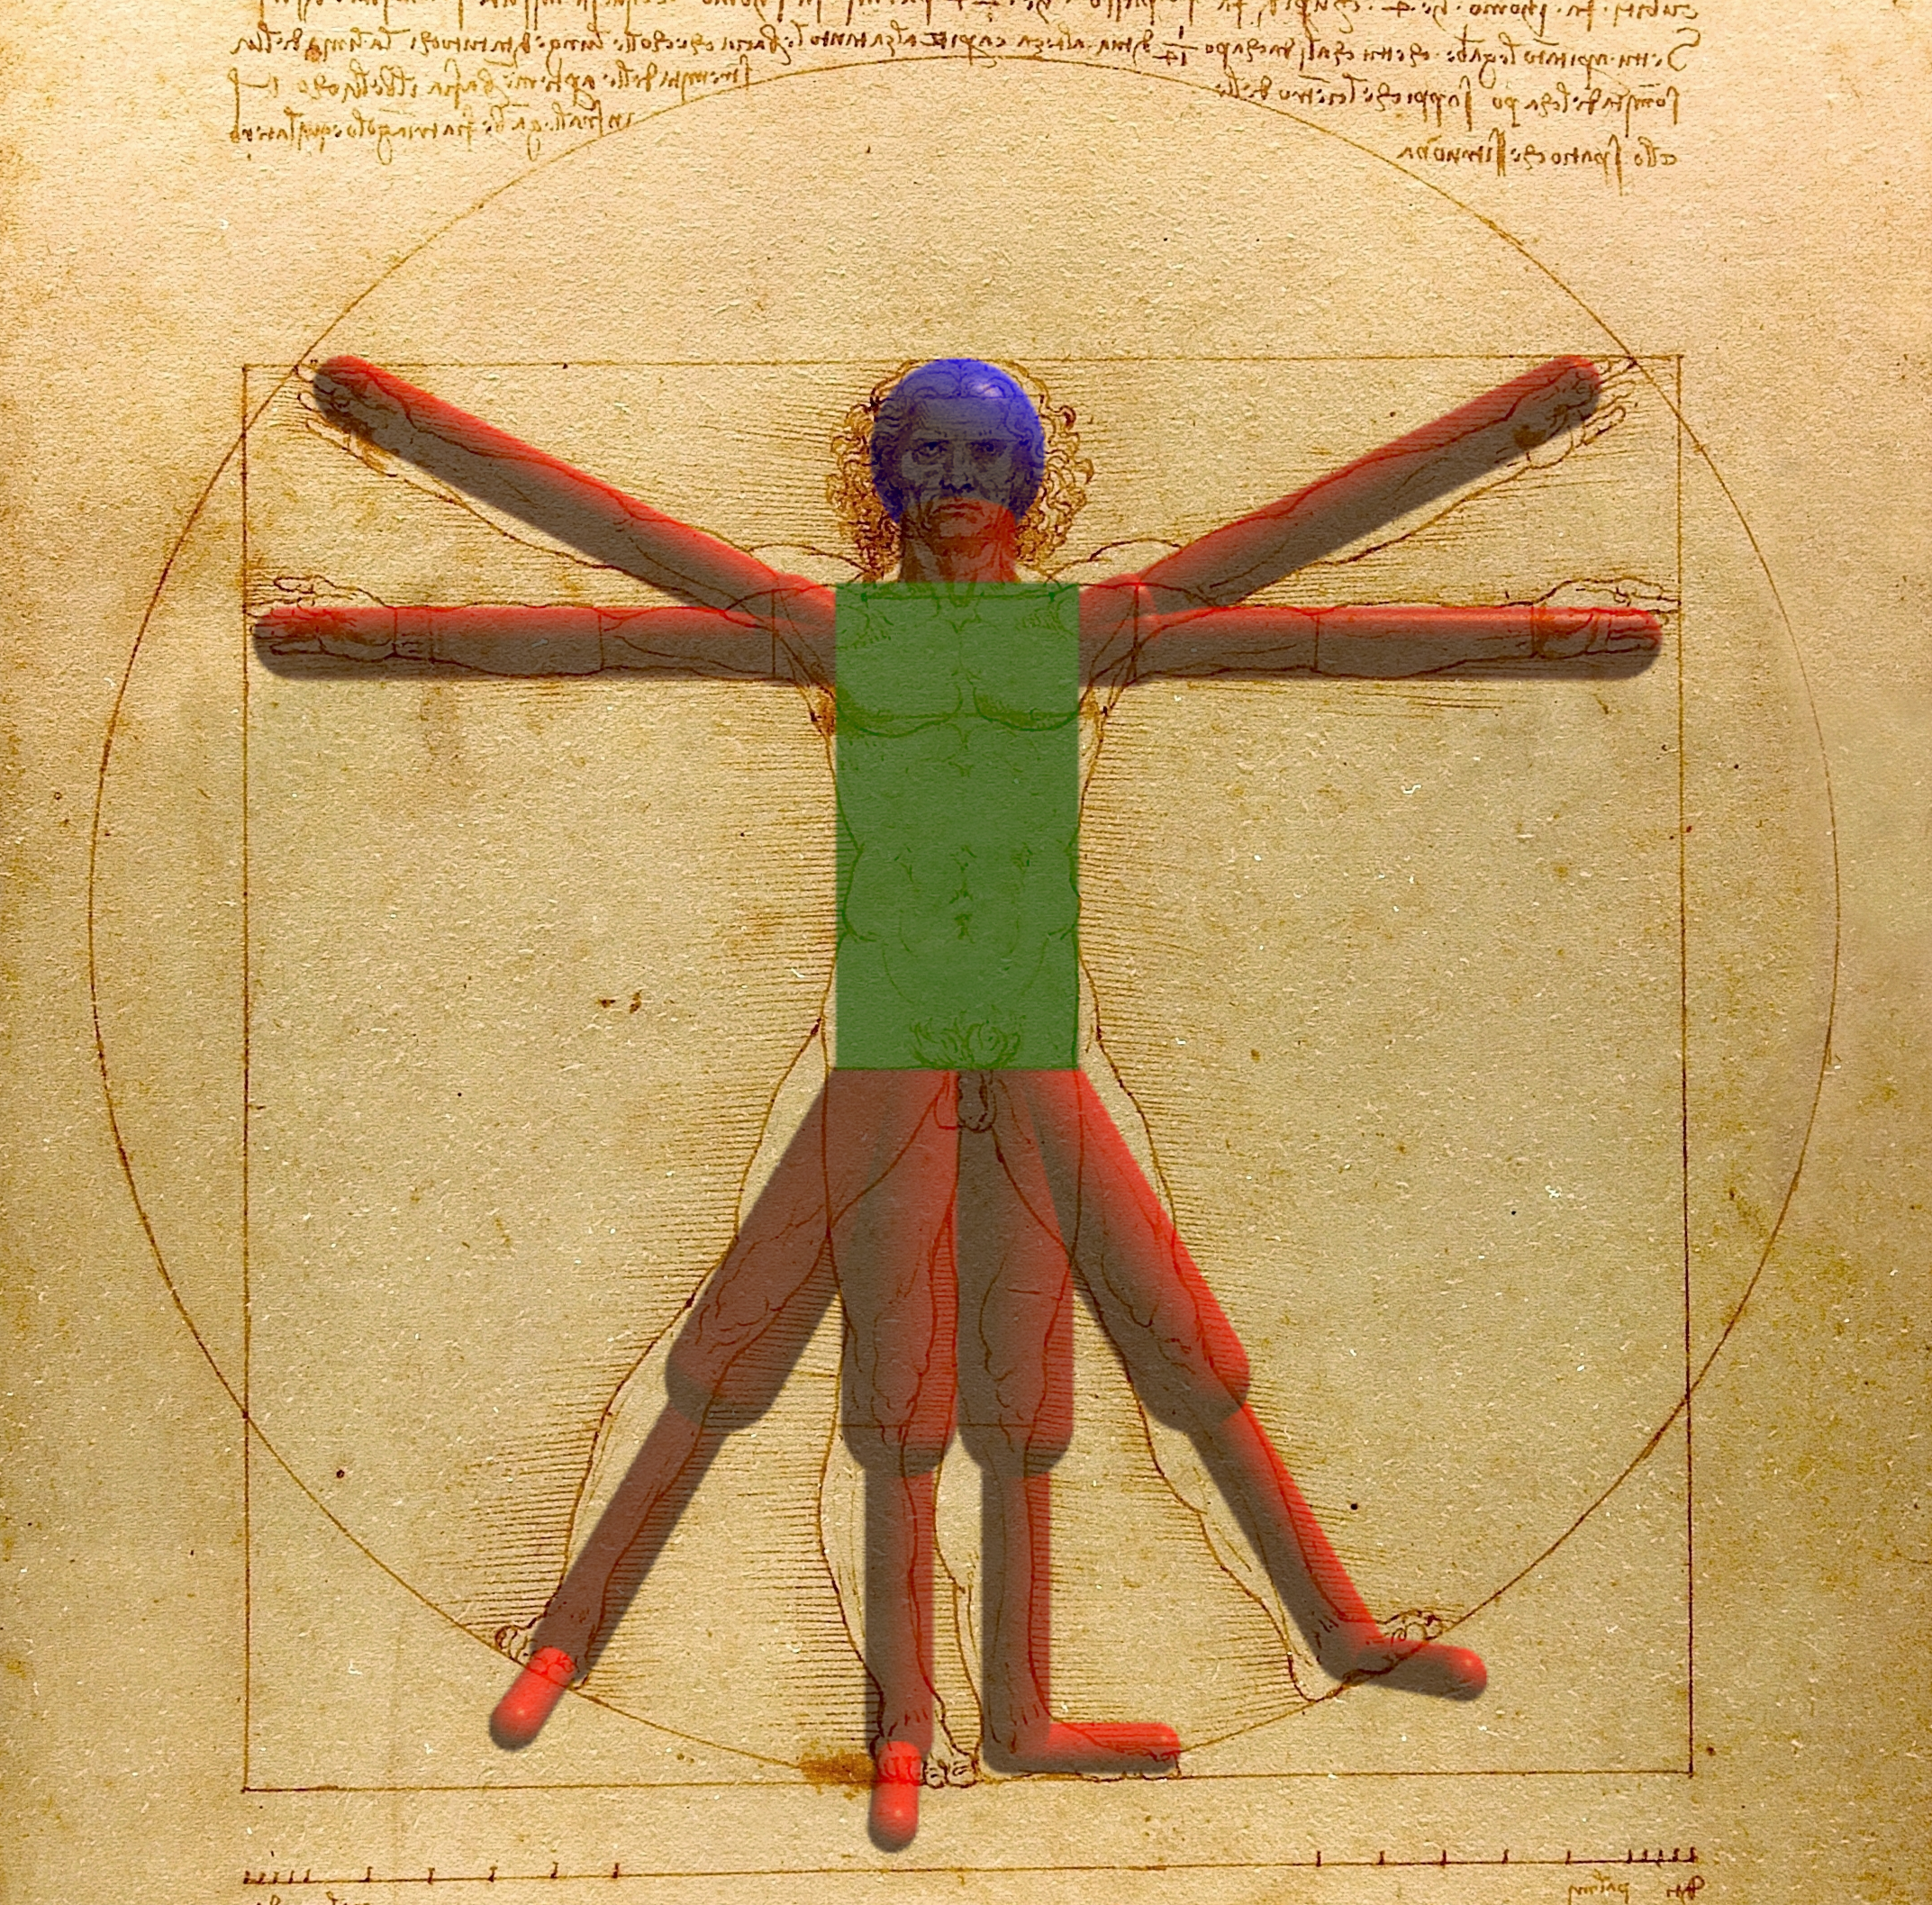
\includegraphics[width=0.6\textwidth,angle=0,clip=]{Vitruvian.png}
}
\caption{\label{Vitruvio:fig}
Our model of the human body compared to the Vitruvian Man by Leonardo da Vinci.
}
\end{figure}
As anticipate we built our body using as base shapes spheres, parallelepipeds and capsules. A direct comparison between our model of the body and the Vitruvian Man can be seen in Fig. \ref{Vitruvio:fig}. The numerical details of our body are available on GitHub at \url{https://github.com/Cr3sp1/RainSimulation/tree/main/Bodies}.
Now that we have our body we have to make it move. We chose to study two regimes of motion: walking and running. 
We decided to model both walking and running with periodic rotations of the limbs around their respective joints. For simplicity's sake we will approximate the periodic time evolution of angles of the joints as sinusoids. 
We decided to model walking as a simple oscillation of the arms and legs. To make sure our dynamic body at least resembles a real human being we refer to articles on the biomechanics of walking and running for the amplitudes and relative phases of our sinusoids.
Provioamo daiiii

\newpage
\section{Technical implementation} \label{technical:sec}



\newpage
\section{Results} \label{results:sec}





\newpage
\section{Discussion and Conclusion}



%------------------------------------------------------------------
%  BIBLIOGRAPHY
%------------------------------------------------------------------
\clearpage  % this may be useful in exceptional cases, e.g. here

\addcontentsline{toc}{section}{References}
\begin{thebibliography}{9}

% note that the references must be listed in the same order as they are cited
% in the text above:
\bibitem{Deakin} 
B. L. Schwartz, M. A. B. Deakin, Math. Mag. {\bf 46}, 272 (1973).

\bibitem{Hailman}
D. Hailman, B. Torrents,  Math. Mag. {\bf 82:4}, 266 (2009).

\bibitem{Bocci}
F. Bocci,  Eur. J. Phys. {\bf 33}, 1321 (2012).

\bibitem{Kroetz}
T. Kroetz, Rev. Bras. Ens. Fis. {\bf 31}, 4 (2012).

\bibitem{Pournin}
L. Pournin, M. Weber, M. Tsukahara, J. A. Ferrez, M. Ramaioli, T. M. Liebling, Granular Matter {\bf 7}, 119 (2005).

\bibitem{Lay} 
D. C. Lay, S. R. Lay, J. J. McDonald,
{\it Linear algebra and its applications, 5th ed.} (Pearson Education, 2014).

\bibitem{Schneider} 
R. Schneider,
{\it Convex bodies: the Brunn–Minkowski theory} (Cambridge Univ. Press, 1993).

\bibitem{Huang}
P. Huang, S. Pan, Y. Yang, Discrete Comput. Geom. {\bf 54}, 728 (2015).

\bibitem{DaVinci}
L. da Vinci, {\it Uomo vitruviano} (1490).

\bibitem{Yegian}
A. K. Yegian, Y. Tucker, S. Gillinov, D. E. Lieberman, J. Exp. Biol. {\bf 220}, 13 (2019) 

\bibitem{Cavanagh}
P. R. Cavanagh, Foot Ankle {\bf 7}, 197 (1987)

\bibitem{Zee}
T. J. van der Zee , E. M. Mundinger, A. D. Kuo1,  Sci Data {\bf 9}, 704 (2022)

\bibitem{Santos}
 A. F. dos Santos, T. H. Nakagawa, G. Y. Nakashima, C. D. Maciel, F. Serrão, Int. J. Sports. Me. {\bf 37}, 369 (2016)


\end{thebibliography}


\end{document}
